\documentclass{article}


\topmargin=-0.45in      %
\evensidemargin=0in     %
\oddsidemargin=0in      %
\textwidth=6.5in        %
\textheight=9.0in       %
\headsep=0.25in         %


\usepackage{graphicx,float,wrapfig}
\usepackage{moreverb} % monospace
\usepackage{fancyhdr} % fancy header 
\usepackage{lastpage} % last page 
\usepackage{setspace} % line spacing
\usepackage{amsmath,amsfonts,amsthm,amssymb}  % math fonts 
\usepackage{tabularx} % advanced tables
\usepackage[unicode=true] {hyperref}
%%% default Rstudio packages %%%

\usepackage[sort]{natbib}  %% will alpha/numeric in order inline
	\setcitestyle{aysep={}} %% no year, comma just year
	
	
\newcommand{\hmwkCourse}{ \textbf{STATS 419 Survey of Multivariate Analysis} }
\newcommand{\hmwkCourseShort}{STATS419}
\newcommand{\hmwkTitle}{Week 03 Assignment}
\newcommand{\hmwkAuthor}{joshua Bennett}
\newcommand{\hmwkEmail}{joshua.r.bennett@wsu.edu}
\newcommand{\hmwkWSU}{[11373111]}
\newcommand{\hmwkInstructor}{Instructor: Monte J. Shaffer}
\newcommand{\hmwkDate}{16 September 2020}


\pagestyle{fancy}   
\lhead{\hmwkCourseShort}
\chead{\hmwkTitle}
\rhead{\hmwkAuthor}
\lfoot{}
\cfoot{Page\ \thepage\ of\ \protect\pageref{LastPage}}
\rfoot{}



\title{\hmwkCourse \\ \hmwkTitle}
\author{\hmwkAuthor \\ (\hmwkEmail) \\ \hmwkWSU \\[0.5in] \hmwkInstructor }
\date{\hmwkDate}


\usepackage{titling}
\pretitle{\begin{flushright}\LARGE}
\posttitle{\par\end{flushright}\vskip 0.5em}
\preauthor{\begin{flushright}\large \lineskip 0.5em}
\postauthor{\par\end{flushright}}
\predate{\begin{flushright}\large}
\postdate{\par\end{flushright}}


%\tracingall



\begin{document}

\maketitle

%\begin{abstract}
%The abstract text goes here.
%\end{abstract}

\section{Introduction}
Here is the text\footnote{Here is a footnote} of your introduction.

Malcolm Gladwell talks about outliers \citep{Gladwell:2008}.

\begin{equation}
    \label{simple_equation}
    \alpha = \sqrt{ \beta }
\end{equation}

\subsection{Subsection Heading Here}
Write your subsection text here.

\begin{figure}
    \centering
    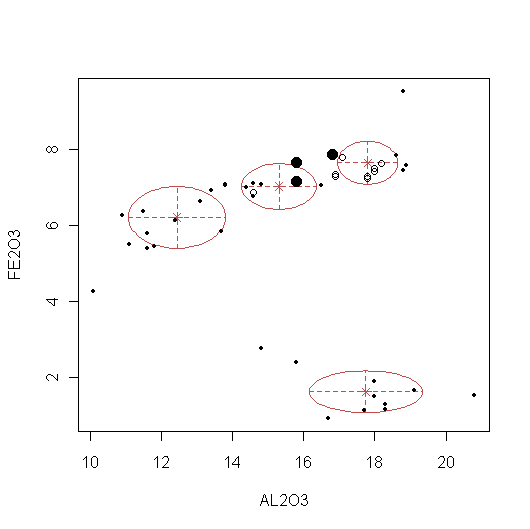
\includegraphics[width=3.0in] {C:/Users/Galac/Desktop/git419/Stats419_FALL2020/LateX/full-example/graphics/myfigure}
   
    \caption{Simulation Results}
    \label{simulationfigure}
\end{figure}


\begin{figure}
    \centering
    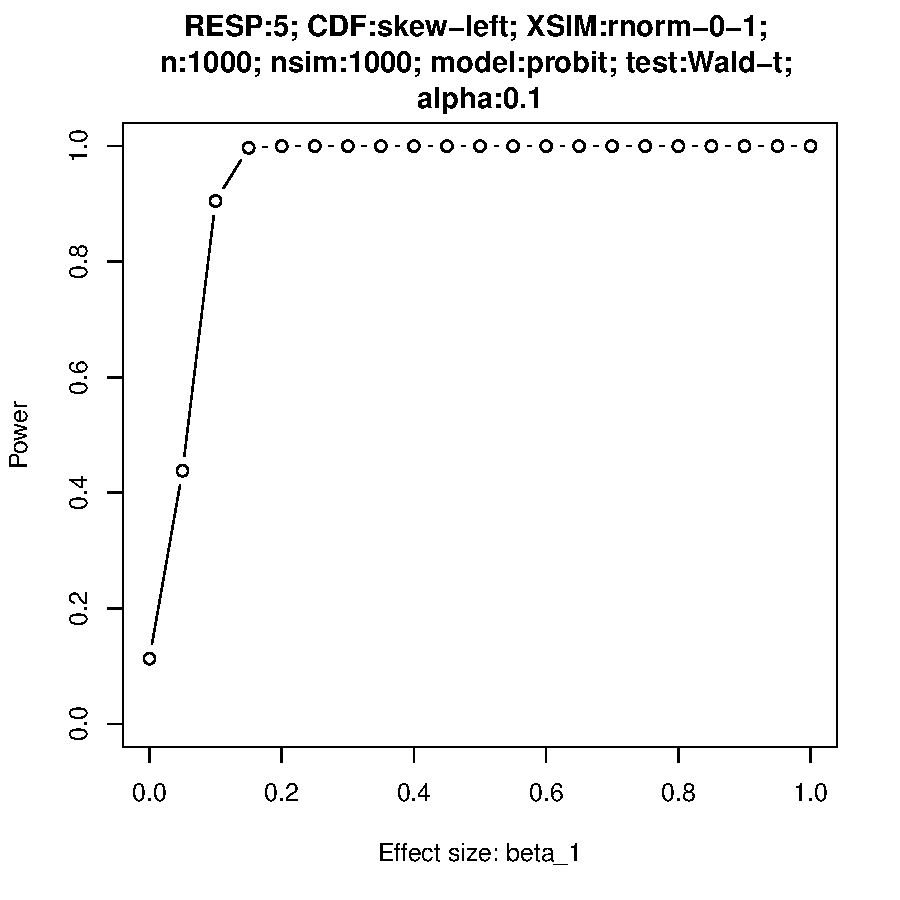
\includegraphics[width=3.0in] {C:/Users/Galac/Desktop/git419/Stats419_FALL2020/LateX/full-example/graphics/pdffigure}
    \caption{Simulation Results PDF}
    \label{simulationfigurepdf}
\end{figure}

\section{Conclusion}
Write your conclusion here.

$body$


\newpage
\bibliographystyle{biblio/chicagoAMA}
\bibliography{biblio/master} % this is master.bib located in the biblio subfolder ... you could have multiple files here if need be ... one is easier ...


\end{document}